%package list
\documentclass{article}
\usepackage[top=3cm, bottom=3cm, outer=3cm, inner=3cm]{geometry}
\usepackage{graphicx}
\usepackage{url}
%\usepackage{cite}
\usepackage{hyperref}
\usepackage{array}
\usepackage{multicol}
\newcolumntype{x}[1]{>{\centering\arraybackslash\hspace{0pt}}p{#1}}
\usepackage{natbib}
\usepackage{pdfpages}
\usepackage{multirow}
\usepackage{float}
\usepackage[normalem]{ulem}
\useunder{\uline}{\ul}{}


%%%%%%%%%%%%%%%%%%%%%%%%%%%%%%%%%%%%%%%%%%%%%%%%%%%%%%%%%%%%%%%%%%%%%%%%%%%%
%%%%%%%%%%%%%%%%%%%%%%%%%%%%%%%%%%%%%%%%%%%%%%%%%%%%%%%%%%%%%%%%%%%%%%%%%%%%
\newcommand{\csemail}{vmachacaa@unsa.edu.pe}
\newcommand{\csdocente}{Vicente Machaca Arceda}
\newcommand{\cscurso}{Algoritmos y Estructura de Datos}
\newcommand{\csuniversidad}{Universidad Nacional de San Agustín}
\newcommand{\csescuela}{Maestría en Ciencia de la Computación}
\newcommand{\cspracnr}{01}
\newcommand{\cstema}{--}
%%%%%%%%%%%%%%%%%%%%%%%%%%%%%%%%%%%%%%%%%%%%%%%%%%%%%%%%%%%%%%%%%%%%%%%%%%%%
%%%%%%%%%%%%%%%%%%%%%%%%%%%%%%%%%%%%%%%%%%%%%%%%%%%%%%%%%%%%%%%%%%%%%%%%%%%%


\usepackage[english,spanish]{babel}
\usepackage[utf8]{inputenc}
\AtBeginDocument{\selectlanguage{spanish}}
\renewcommand{\figurename}{Figura}
\renewcommand{\refname}{Referencias}
\renewcommand{\tablename}{Tabla} %esto no funciona cuando se usa babel
\AtBeginDocument{%
	\renewcommand\tablename{Tabla}
}

\usepackage{fancyhdr}
\pagestyle{fancy}
\fancyhf{}
\setlength{\headheight}{30pt}
\renewcommand{\headrulewidth}{1pt}
\renewcommand{\footrulewidth}{1pt}
\fancyhead[L]{\raisebox{-0.2\height}{
\includegraphics[width=3cm]{img/logo_unsa}}}
\fancyhead[C]{}
\fancyhead[R]{\fontsize{7}{7}\selectfont	\csuniversidad \\ \csescuela \\ \textbf{\cscurso} }
\fancyfoot[L]{MSc. Vicente Machaca}
\fancyfoot[C]{\cscurso}
\fancyfoot[R]{Página \thepage}


\begin{document}
	
	\vspace*{10px}
	
	\begin{center}	
		\fontsize{17}{17} \textbf{ Práctica \cspracnr}
	\end{center}
	%\centerline{\textbf{\underline{\Large Título: Informe de revisión del estado del arte}}}
	%\vspace*{0.5cm}
	

	\begin{table}[h]
		\begin{tabular}{|x{4.7cm}|x{4.8cm}|x{4.8cm}|}
			\hline
			\textbf{DOCENTE} & \textbf{CARRERA}  & \textbf{CURSO}   \\
			\hline
			\csdocente & \csescuela & \cscurso    \\
			\hline
		\end{tabular}
	\end{table}	
	
	
	\begin{table}[h]
		\begin{tabular}{|x{4.7cm}|x{4.8cm}|x{4.8cm}|}
			\hline
			\textbf{PRÁCTICA} & \textbf{TEMA}  & \textbf{DURACIÓN}   \\
			\hline
			\cspracnr & \cstema & 3 horas   \\
			\hline
		\end{tabular}
	\end{table}
	
	
	\section{Datos de los estudiantes}
	\begin{itemize}
		\item Grupo: 2
		\item Integrantes:
		\begin{itemize}
			\item EDER ALONSO AMPUERO ATAMARI
			\item HOWARD FERNANDO ARANZAMENDI MORALES
            \item JOSE EDISON PEREZ MAMANI
            \item HENRRY IVAN ARIAS MAMANI
		\end{itemize}		
	\end{itemize}
        \section{Url GIT}
      Repositorio Github: https://github.com/hAriasm/AlgoritmoOrdenamiento

	\section{Algoritmo de Ordenamiento}\label{sec:ejercicios}



     \subsection{MergeSort}
    \paragraph{}
    El Merge Sort es un algoritmo recursivo bastante eficiente para ordenar un array, que tiene un orden de complejidad O(nlogn) al igual que Quick Sort. fue desarrollado en 1945 por John Von Neumann.

    El Merge Sort está basado en la técnica de diseño de algoritmos Divide y Vencerás, esta técnica consiste en dividir el problema a resolver en sub problemas del mismo tipo que a su vez se dividirán, mientras no sean suficientemente  pequeños o triviales.
    \begin{figure}[h!]
        \centering
        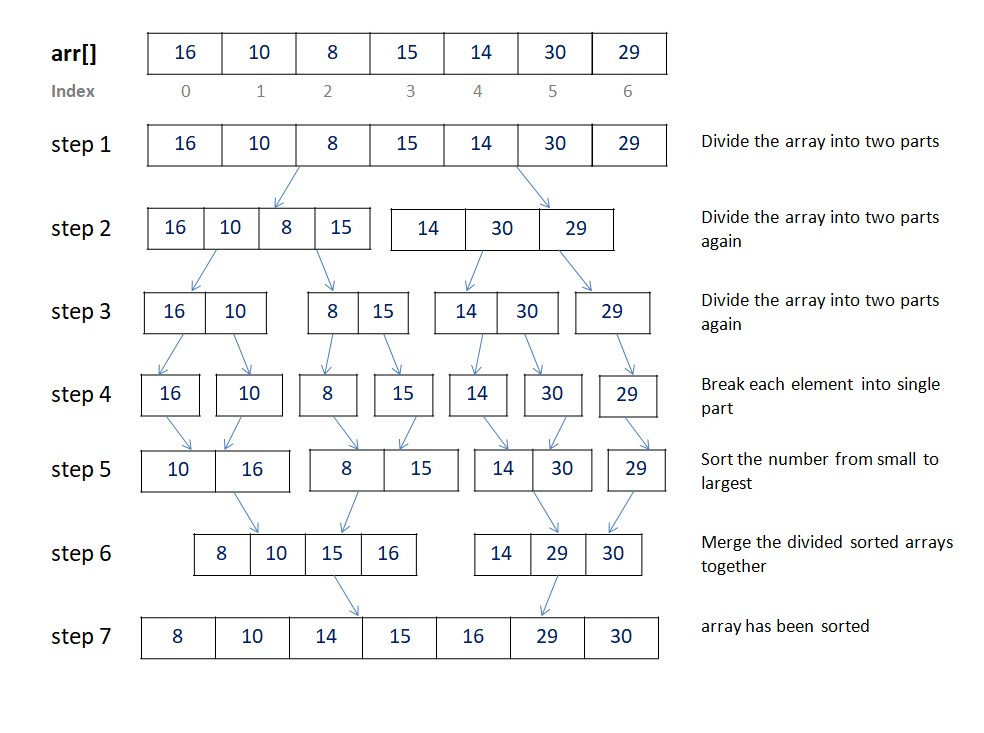
\includegraphics[width=12cm]{img/mergesort.png}
        \caption{Estrategia que sigue algoritmo para ordenar una secuencia S de n elementos}
        \label{fig:mergesort}
    \end {figure}
    \begin{itemize}
        \item Si S tiene uno o ningún elemento, está ordenada.
        \item Si S tiene al menos dos elementos se divide en dos secuencias S1 y S2.
        \item S1 contiene los primeros n/2 elementos y S2 los restantes.
        \item Ordenar S1 y S2, aplicando recursivamente este procedimiento
        \item Mezclar S1 y S2 en S, de forma que ya S1 y S2 estén ordenados
        \item Veamos ahora como sería la estrategia para mezclar las secuencias:
    \end{itemize}
    \paragraph {}
    Se tienen referencias al principio de cada una de las secuencias a mezclar (S1 y S2). Mientras en alguna secuencia queden elementos, se inserta en la secuencia resultante (S) el menor de los elementos referenciados y se avanza esa referencia una posición.
      \subsubsection{Gráfica MergeSort}
        \begin{figure}[h!]
            \centering
            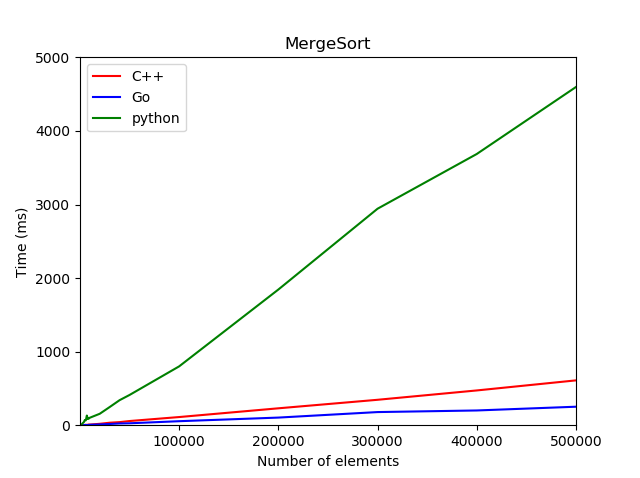
\includegraphics[width=12cm]{img/mergeSort_1.png}
            \caption{Estrategia que sigue algoritmo para ordenar una secuencia S de n elementos}
            \label{fig:mergesort}
        \end {figure}
        \begin{figure}[h!]
            \centering
            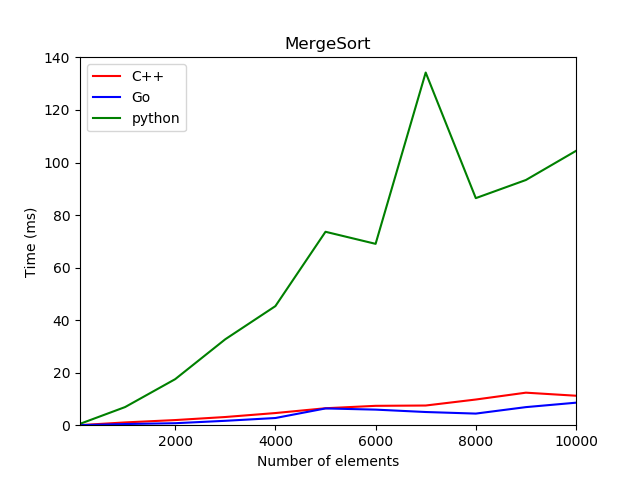
\includegraphics[width=12cm]{img/mergeSort_2.png}
            \caption{Estrategia que sigue algoritmo para ordenar una secuencia S de n elementos}
            \label{fig:mergesort}
        \end {figure}
    \begin{table}[]
        \begin{tabular}{|c|c|c|c|c|c|c|c| }
            \hline
            \multicolumn{8}{c}{Algoritmo: Merge Sort} \\  
            \multicolumn{4}{|c|}{} & \multicolumn{4}{c|}{Lenguaje: C++} \\  
              N de Datos &     t1    &  t2         &  t3          &   t4        &    t5     &   Promedio(t)       & desv. s. \\  
                100	    &0.1487	&0.0874	&0.1071	&0.0755	&0.11	&0.10574	&0.027912237\\  
                1000	&1.2993	&0.8411	&0.9458	&1.2623	&1.3617	&1.14204	&0.232657856\\ \hline
                2000	&1.743	&1.5607	&2.0408	&2.788	&2.0492	&2.03634	&0.468364119\\ \hline
                3000	&3.1413	&3.3076	&3.7817	&3.0035	&2.7599	&3.1988	&0.382652388\\ \hline
                4000	&3.5795	&3.8921	&3.898	&5.6032	&6.5539	&4.70534	&1.304223862\\ \hline
                5000	&7.2039	&4.8042	&5.7385	&8.846	&6.0797	&6.53446	&1.55125157\\ \hline
                6000	&7.7235	&5.8136	&8.4027	&5.9593	&9.3577	&7.45136	&1.542865924\\ \hline
                7000	&7.6291	&7.3039	&8.143	&7.7513	&7.0229	&7.57004	&0.428607954\\ \hline
                8000	&10.2886	&8.213	&10.2271	&11.791	&8.7372	&9.85138	&1.415992469\\ \hline
                9000	&9.2446	&18.651	&13.6912	&9.715	&10.9793	&12.45622	&3.87009553\\ \hline
                10000	&11.0627	&9.9283	&11.7518	&11.2358	&12.4952	&11.29476	&0.945315134\\ \hline
                20000	&21.3784	&22.2088	&21.4662	&23.3717	&21.1154	&21.9081	&0.913342274\\ \hline
                30000	&33.4084	&32.9699	&44.6192	&35.4287	&36.7651	&36.63826	&4.71867004\\ \hline
                40000	&48.641	&44.7479	&46.0825	&42.4689	&41.8431	&44.75668	&2.76444856\\ \hline
                50000	&65.7168	&54.3054	&60.5532	&58.114	&59.0799	&59.55386	&4.148031978\\ \hline
                100000	&114.8989	&110.1903	&113.0493	&112.5492	&117.7412	&113.68578	&2.821054449\\ \hline
                200000	&234.386	    & 229.6066	&230.8164	&227.1946	&240.2287	&232.44646	&5.065298824\\ \hline
                300000	&353.5663	&349.7128	&344.6946	&337.0085	&356.1979	&348.23602	&7.625338651\\ \hline
                400000	&478.9285	&463.8541	&474.8911	&481.0437	&477.0424	&475.15196	&6.713015465\\ \hline
                500000	&589.1112	&580.0919	&593.2032	&591.8553	&705.3167	&611.91566	&52.46218536\\ \hline
        \end{tabular}
        \caption{Tabla de resultados Merge Sort con C++}
        \label{tab:mergeSortC}
    \end{table}



        \begin{table}[]
        \begin{tabular}{|c|c|c|c|c|c|c|c| }
            \hline
            \multicolumn{8}{|c|}{Algoritmo: Merge Sort} \\ \hline
            \multicolumn{4}{|c|}{} & \multicolumn{4}{c|}{Lenguaje:GO} \\ \hline
              N de Datos &     t1    &  t2         &  t3          &   t4        &    t5     &   Promedio(t)       & desv. s. \\ \hline
            100&	0.5074&	0	&0	&0	&0	&0.10148	&0.226916178\\ \hline
            1000&	0.5219	&0.5233	&0.5287	&0.5202	&0.54	&0.52682	&0.00802602\\ \hline
            2000	&1.0521	&1.0386	&1.0428	&0.5246	&0.5372	&0.83906	&0.281387985\\ \hline
            3000	&2.2709	&1.558	&2.2751	&1.0488	&1.6232	&1.7552	&0.522387619\\ \hline
            4000	&2.6873	&2.9265	&3.3548	&3.0641	&2.0366	&2.81386	&0.497009671\\ \hline
            5000	&6.1804	&6.8845	&5.8358	&6.5053	&6.9	  & 6.4612	&0.459251277\\ \hline
            6000	&2.715	&7.7319	&2.0867	&8.5517	&8.9547	&6.008	&3.329629277\\ \hline
            7000	&4.2708	&3.1435	&8.8315	&2.6065	&6.6433&	5.09912	&2.599945692\\ \hline
            8000	&3.5225	&3.8262	&2.0935	&8.3747	&4.678	&4.49898	&2.358269166\\ \hline
            9000	&4.9988	&7.0219	&7.3279	&7.135	&8.3189&	6.9605	&1.21065276\\ \hline
            10000	&3.996	&21.9886	&3.0013	&9.8411	&4.4007	&8.64554	&7.920873498\\ \hline
            20000	&11.9906	&17.9899	&9.9957	&13.9928	&11.8163	&13.15706	&3.049887997\\ \hline
            30000	&16.9902	&24.9881	&14.9913	&17.8918	&21.8538	&19.34304	&4.023375847\\ \hline
            40000	&27.9822	&26.9853	&22.9909	&28.0106	&24.9855	&26.1909	  &2.170490976\\ \hline
            50000	&30.9813	&26.6258	&30.8381	&23.6203	&32.9822&	29.00954	&3.799329573\\ \hline
            100000	&52.5777	&63.9633	&56.2067	&56.4835	&57.2278	&57.2918&	4.140245704\\ \hline
            200000&	96.7328	  &   107.6231	&107.2718	&110.1763	&110.3102	&106.42284	&5.59594188\\ \hline
            300000	&153.1654	&161.9075	&147.6206	&273.9708	&170.0507	&181.343	    &52.47938032\\ \hline
            400000&	180.8225&	195.6433	&192.2494	&218.5503	&228.3242	&203.11794	&19.65067001\\ \hline
            500000	&226.1258&	261.0595	&266.9817	&267.5833	&248.8818	&254.12642	&17.36342565\\ \hline

                \end{tabular}
                   \caption{Tabla de resultados Merge Sort con GO}
        \label{tab:mergeSortGO}
    \end{table}
                    \begin{table}[]
        \begin{tabular}{|c|c|c|c|c|c|c|c| }
            \hline
            \multicolumn{8}{|c|}{Algoritmo: Merge Sort} \\ \hline
            \multicolumn{4}{|c|}{} & \multicolumn{4}{c|}{Lenguaje:Python} \\ \hline
              N de Datos &     t1    &  t2         &  t3          &   t4        &    t5     &   Promedio(t)       & desv. s. \\ \hline
                100 &	0.00099802	 &0.001014233	 &0 &	0 &	0.000999451 &	0.602340698	 &0.549895942\\ \hline
                1000 &	0.005995512 &	0.008973598 &	0.007950544 &	0.006989479 &	0.005000591 &	6.981945038	 &1.565546045\\ \hline
                2000 &	0.014994144	 &0.019010305 &	0.025984049 &	0.013988256 &	0.014013529	 &17.59805679	 &5.122967099\\ \hline
                3000 &	0.029980659 &	0.021990776 &	0.051969767 &	0.039978981 &	0.019966602 &	32.7773571	 &13.30882467\\ \hline
                4000	 &0.030983925 &	0.037979603 &	0.072960138 &	0.062963486 &	0.022008896 &	45.37920952	 &21.66831998\\ \hline
                5000 &	0.057966948	 &0.040974855 &	0.122928381 &	0.107444286 &	0.038974047 &	73.6577034	 &39.00787506\\ \hline
                6000 &	0.051971197 &	0.045973539 &	0.103938818 &	0.106939316 &	0.036498547 &	69.06428337	 &33.67727169\\ \hline
                7000 &	0.160906315 &	0.057966471 &	0.296339989 &	0.111934662 &	0.043976307 &	134.2247486	 &101.7966247\\ \hline
                8000 &	0.067960262 &	0.05896616 &	0.099942446 &	0.156917572 &	0.048482656 &	86.45381927 &	43.83627428\\ \hline
                9000 &	0.07095933	 &0.067960978 &	0.096944094 &	0.161907196 &	0.068982124 &	93.35074425 &	40.16448861\\ \hline
                10000 &	0.099942446 &	0.076957464 &	0.108938456 &	0.181349754 &	0.054946661	 &104.4269562	 &47.85513018\\ \hline
                20000 &	0.159907818 &	0.145916224 &	0.155697346 &	0.216875553 &	0.112954617	 &158.2703114	 &37.58327961\\ \hline
                30000 &	0.231253624 &	0.224879026 &	0.239089012 &	0.369790792 &	0.183023691	 &249.6072292 &	70.59820845\\ \hline
                40000 &	0.392888308 &	0.310826063 &	0.274857521 &	0.376797676 &	0.359117985	 &342.8975105	 &48.91171307\\ \hline
                50000 &	0.420777798 &	0.390955448 &	0.371768951 &	0.551683903 &	0.332072973	 &413.4518147	 &83.70759169\\ \hline
                100000 &	0.767641544	 &0.713899851 &	0.910475492 &	0.867524147 &	0.750571966 &	802.0226002	 &83.13742566\\ \hline
                200000 &	1.803967714 &	1.712458849 &	2.245170116 &	1.832188606 &	1.635478973	 &1845.852852 &	236.3506309\\ \hline
                300000 &	3.931644201 &	2.67054534 &	2.755848169 &	2.798952579 &	2.56230402	 &2943.858862	 &559.5422475\\ \hline
                400000 &	3.860989094 &	3.510637999 &	3.683504343 &	3.768096685 &	3.613694191	 &3687.384462	 &135.4046296\\ \hline
                500000 &	4.537797928 &	4.659104586 &	4.622467756 &	4.709950686 &	4.4588449	 &4597.633171 &99.81627618\\ \hline
            \end{tabular}
               \caption{Tabla de resultados Merge Sort con Python}
        \label{tab:mergeSortPython}
    \end{table}
    \subsection{QuickSort}
        \paragraph {}
        Quicksort ha sido históricamente el algoritmo genérico \label[aaaa]{quickSortPython}de ordenamiento más rápido conocido en la práctica. Es un algoritmo recursivo del tipo “divide y vencerás”, es fácil de implementar, que permite, en promedio, ordenar n elementos en un tiempo proporcional a n log n.
        \paragraph {}
        La idea básica es ordenar una lista siguiendo los pasos siguientes: se escoge un elemento arbitrario de la lista y se forman tres grupos; el primer grupo, tiene los elementos menores a aquel que se escogió; el segundo, los elementos iguales que el escogido; y el tercero, tiene los elementos más grandes. De forma recursiva, se ordenan el primer y el tercer grupo; luego, se concatenan todos los grupos.
        \paragraph {}
        Este método fue creado por el científico británico Charles Antony Richard Hoare, también conocido como Tony Hoare en 1960, su algoritmo Quicksort es el algoritmo de ordenamiento más ampliamente utilizado en el mundo.
           \begin{figure}[h!]
            \centering
            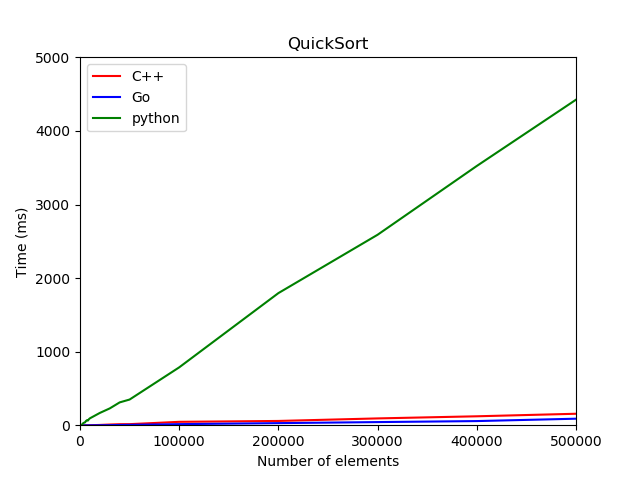
\includegraphics[width=12cm]{img/QuickSort_1.png}
            \caption{Estrategia que sigue algoritmo para ordenar una secuencia S de n elementos}
            \label{fig:mergesort}
        \end {figure}


    \begin{table}[]
        \begin{tabular}{|c|c|c|c|c|c|c|c| }
            \hline
            \multicolumn{8}{|c|}{Algoritmo: Quick Sort} \\ \hline
            \multicolumn{4}{|c|}{} & \multicolumn{4}{c|}{Lenguaje: C++} \\ \hline
              N de Datos &     t1    &  t2         &  t3          &   t4        &    t5     &   Promedio(t)       & desv. s. \\ \hline
                100	    &0.0187	&0.0233	&0.0163	&0.0245	&0.0225	&0.02106	&0.003433366 \\ \hline
                1000	&0.2602	&0.3473	&0.4579	&0.2286	&0.259	&0.3106	&0.09350254 \\ \hline
                2000	&0.733	&0.5807	&0.7085	&0.7691	&0.6711	&0.69248	&0.071973968 \\ \hline
                3000	&0.7919	&0.7924	&0.9621	&1.0846	&1.1932	&0.96484	&0.177582412 \\ \hline
                4000	&1.2483	&1.2782	&1.2328	&1.7202	&1.4819	&1.39228	&0.209010543 \\ \hline
                5000	&2.0514	&1.7369	&2.3129	&1.6202	&2.1261	&1.9695	&0.285161349 \\ \hline
                6000	&2.8691	&2.0011	&2.6279	&2.4449	&2.6059	&2.50978	&0.322206071 \\ \hline
                7000	&3.4611	&2.5416	&2.9049	&3.0544	&2.5433	&2.90106	&0.385479056 \\ \hline
                8000	&3.3108	&3.265	&3.8929	&2.9292	&3.9379	&3.46716	&0.435192133 \\ \hline
                9000	&3.8874	&3.6595	&3.986	&3.4005	&3.9895	&3.78458	&0.253128736 \\ \hline
                10000	&4.784	&4.0452	&3.7409	&6.5858	&3.8669	&4.60456	&1.179029806 \\ \hline
                20000	&12.7512	&10.055	&8.812	&11.8333	&8.1281	&10.31592&	1.958918178 \\ \hline
                30000	&12.8663	&12.6601	&23.3719	&15.1841	&13.4952	&15.51552&	4.502389055 \\ \hline
                40000	&18.1782	&16.4566	&20.842	&20.9858	&21.1016	&19.51284&	2.096562822 \\ \hline
                50000	&32.1925	&21.2544	&38.008	&24.691	&35.0562	&30.24042&	7.05128127 \\ \hline
                100000	&60.913	&49.2804	&48.2738	&46.4789	&53.1548	&51.62018&	5.740582542 \\ \hline
                200000	&126.1002	&98.1128	    &106.289	    &101.0139	&109.0098&	108.10514&	10.93242313 \\ \hline
                300000	&189.3729	&165.117	    &153.6852	&155.4696	&160.9269&	164.91432&	14.4001615 \\ \hline
                400000	&255.2373	&213.9224	&225.0151	&215.6328	&229.8306&	227.92764&	16.62251119 \\ \hline
                500000	&306.2959	&275.6362	&280.8843	&283.1553	&308.869	 &    290.96814&	15.43675563 \\ \hline
        \end{tabular}
           \caption{Tabla de resultados Quick Sort con C++}
        \label{tab:quickSortC}
    \end{table}
        \begin{table}[]
        \begin{tabular}{|c|c|c|c|c|c|c|c| }
            \hline
            \multicolumn{8}{|c|}{Algoritmo: Quick Sort} \\ \hline
            \multicolumn{4}{|c|}{} & \multicolumn{4}{c|}{Lenguaje: GO} \\ \hline
              N de Datos &     t1    &  t2         &  t3          &   t4        &    t5     &   Promedio(t)       & desv. s. \\ \hline
                100	&0.0156&0	&0	&0	&0	&0.00312	&0.006976532\\ \hline
                1000	&0	&0	&0.1399	&0.2501	&0.3944	&0.15688	&0.169275447\\ \hline
                2000	&0.5932	&0	&0.5816	&0.523	&0.5053	&0.44062	&0.249134486\\ \hline
                3000	&0.5216	&0.7014	&0.5219	&0.5225	&0.525	&0.55848	&0.079905926\\ \hline
                4000	&0.5286	&0.5174	&1.3393	&1.0046	&2.0038	&1.07874	&0.621868329\\ \hline
                5000	&1.08	&1.0216	&1.0381	&1.5512	&1.0355	&1.14528	&0.227962973\\ \hline
                6000	&1.0445	&1.5569	&1.5466	&1.6007	&2.0228	&1.5543	&0.346989661\\ \hline
                7000	&2.6622	&1.0502	&5.1495	&2.1433	&1.0329	&2.40762	&1.687085216\\ \hline
                8000	&2.871	&1.5809	&2.1138	&1.0314	&1.5505	&1.82952	&0.696806162\\ \hline
                9000	&1.5823	&2.3895	&1.5512	&1.5473	&2.4434	&1.90274	&0.469533889\\ \hline
                10000	&2.4711	&2.976	&1.5074	&2.9959	&8.6499	&3.72006	&2.821219629\\ \hline
                20000	&6.259	&3.9964	&5.9965	&4.9961	&5.8911	&5.42782	&0.93062222\\ \hline
                30000	&9.3379	&6.996	&9.0586	&8.5519	&10.994	&8.98768	&1.441327259\\ \hline
                40000	&9.9578	&8.9915	&17.1128	&14.9916	&18.2064	&13.85202	&4.173774013\\ \hline
                50000	&17.2317	&18.9895	&26.8295	&19.5135	&21.4947	&20.81178	&3.691291843\\ \hline
                100000	&44.588	&30.9826	&32.9784	&49.9699	&67.3861	&45.181	&14.72115559\\ \hline
                200000	&41.5332	     &159.2225	&100.7466	&114.9337	&138.887	     &111.0646	&44.85898995\\ \hline
                300000	&79.1607	     &150	    &109.679	    &108.9505	&96.2503	     &108.8081	&26.1448754\\ \hline
                400000	&127.1079	&135.2571	&137.8239	&158.002	      &126.1373	&136.86564	&12.85070179\\ \hline
                500000	&167.5356	&171.6628	&189.0014	&183.3456	&164.9439	&175.29786	&10.40701635\\ \hline
        \end{tabular}
           \caption{Tabla de resultados Quick Sort con GO}
        \label{tab:quickSortC}
    \end{table}


            \begin{table}[]
        \begin{tabular}{|c|c|c|c|c|c|c|c| }
            \hline
            \multicolumn{8}{|c|}{Algoritmo: Quick Sort} \\ \hline
            \multicolumn{4}{|c|}{} & \multicolumn{4}{c|}{Lenguaje: Python} \\ \hline
              N de Datos &     t1    &  t2         &  t3          &   t4        &    t5     &   Promedio(t)       & desv. s. \\ \hline
100	&0	&0	&0.000998735&	0.000998974&	0	&0.399541855	&0.547095223\\ \hline
1000	&0.009994268	&0.011993647	&0.016989946	&0.012970448&	0.005999088	&11.58947945	&4.032140823\\ \hline
2000	&0.029981136	&0.023008108	&0.064962626	&0.033980846	&0.052969933	&40.98052979	&17.40601087\\ \hline
3000	&0.101940393	&0.039955139	&0.060964823	&0.059965849	&0.068959475	&66.35713577	&22.58279991\\ \hline
4000	&0.108939171	&0.042973995	&0.136921167	&0.138915539	&0.125930548	&110.736084	&39.70372012\\ \hline
5000	&0.09194541	&0.051973581	&0.160906792	&.116374493	&0.15090847	&114.4217491	&44.44353917\\ \hline
6000	&0.08195281	&0.07095933	&0.15591073	&0.166904211	&0.185434818	&132.2323799	&52.14336347\\ \hline
7000	&0.102569818	&0.077952385	&0.186402321	&0.167904139	&0.202881813	&147.5420952	&54.43447383\\ \hline
8000	&0.09894228	&0.09294796	&0.15191102	&0.222416639	&0.130926132	&139.4288063	&52.23674347\\ \hline
9000	&0.117349625	&0.10094142	&0.207879543	&0.13805747	&0.220872641	&157.0201397	&54.18019991\\ \hline
10000	&0.225871801	&0.102969408	&0.158908844	&0.216874361	&0.165904284	&174.1057396	&49.66756315\\ \hline
20000	&0.241859674	&0.246831179	&0.359793901	&0.27782321	&0.340345383	&293.3306694	&54.03631127\\ \hline
30000	&0.406769276	&0.36578846	&0.42777729	&0.49301672	&0.394275188	&417.5253868	&47.79387554\\ \hline
40000	&0.529407501	&0.572183132	&0.62464118	&0.566672802	&0.664618015	&591.5045261	&53.12624451\\ \hline
50000	&0.6591959	&0.721586943	&0.773604155	&0.776862621	&0.686623096	&723.574543	&52.09738708\\ \hline
100000	&1.371208668	&1.430203676	&1.544603109	&1.464600325	&1.51870966	&1465.865088	&69.32784174\\ \hline
200000	&3.062305212	&3.088241339	&3.135392666	&3.151999712	&2.980718374	&3083.731461	&67.86116961\\ \hline
300000	&4.930557966	&4.727021456	&4.675037146	&4.993543625	&4.923748016	&4849.981642	&139.882852\\ \hline
400000	&7.751039982	&6.572371244	&6.236221552	&6.337382078	&6.679156542	&6715.23428	&605.5638658\\ \hline
500000	&8.079737902	&9.067592859	&8.209435701	&8.917642117	&8.596114874	&8574.104691	&429.946211\\ \hline

             \end{tabular}
                        \caption{Tabla de resultados Quick Sort con Python}
        \label{tab:quickSortPython}
    \end{table}

    \subsection{HeapSort}
        \paragraph {}
        Heapsort ordena un vector de n elementos construyendo un heap con los n elementos y extrayéndolos a continuación, uno a uno del heap. El propio vector que almacena a los n elementos se emplea para construir el heap, de modo que heapsort actúa in-situ y sólo requiere un espacio auxiliar de memoria constante. El coste de este algoritmo es O(nlogn)(incluso en caso mejor) si todos los elementos son diferentes.
        \paragraph {}
        En la práctica su coste es superior al de quicksort, ya que el factor constante multiplicativo del término nlogn es mayor.

            \begin{figure}[h!]
            \centering
            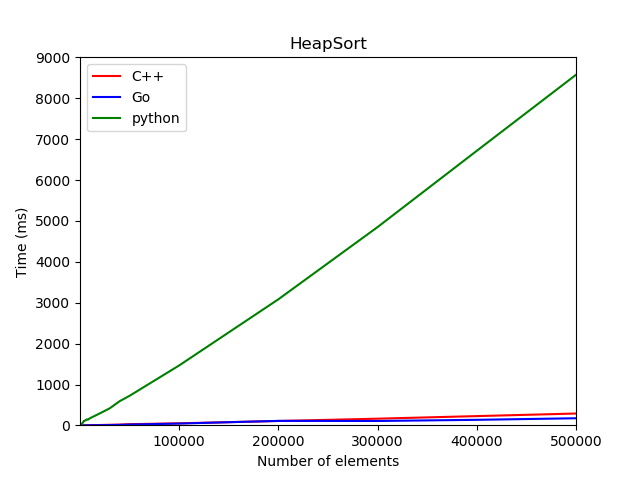
\includegraphics[width=12cm]{img/HeapSort_1.png}
            \caption{Estrategia que sigue algoritmo para ordenar una secuencia S de n elementos}
            \label{fig:heapsort}
        \end {figure}

            \begin{table}[]
        \begin{tabular}{|c|c|c|c|c|c|c|c| }
            \hline
            \multicolumn{8}{|c|}{Algoritmo: Heap Sort} \\ \hline
            \multicolumn{4}{|c|}{} & \multicolumn{4}{c|}{Lenguaje: C++} \\ \hline
              N de Datos &     t1    &  t2         &  t3          &   t4        &    t5     &   Promedio(t)       & desv. s. \\ \hline
                 100	&0.0187	&0.0233	&0.0163	&0.0245	&0.0225	&0.02106	&0.003433366\\ \hline
                1000	&0.2602	&0.3473	&0.4579	&0.2286	&0.259	&0.3106	&0.09350254\\ \hline
                2000	&0.733	&0.5807	&0.7085	&0.7691	&0.6711	&0.69248	&0.071973968\\ \hline
                3000	&0.7919	&0.7924	&0.9621	&1.0846	&1.1932	&0.96484	&0.177582412\\ \hline
                4000	&1.2483	&1.2782	&1.2328	&1.7202	&1.4819	&1.39228	&0.209010543\\ \hline
                5000	&2.0514	&1.7369	&2.3129	&1.6202	&2.1261	&1.9695	&0.285161349\\ \hline
                6000	&2.8691	&2.0011	&2.6279	&2.4449	&2.6059	&2.50978	&0.322206071\\ \hline
                7000	&3.4611	&2.5416	&2.9049	&3.0544	&2.5433	&2.90106	&0.385479056\\ \hline
                8000	&3.3108	&3.265	&3.8929	&2.9292	&3.9379	&3.46716	&0.435192133\\ \hline
                9000	&3.8874	&3.6595	&3.986	&3.4005	&3.9895	&3.78458	&0.253128736\\ \hline
                10000	&4.784	&4.0452	&3.7409	&6.5858	&3.8669	&4.60456	&1.179029806\\ \hline
                20000	&12.7512	&10.055	&8.812	&11.8333	&8.1281	&10.31592&	1.958918178\\ \hline
                30000	&12.8663	&12.6601	&23.3719	&15.1841	&13.4952	&15.51552&	4.502389055\\ \hline
                40000	&18.1782	&16.4566	&20.842	&20.9858	&21.1016	&19.51284&	2.096562822\\ \hline
                50000	&32.1925	&21.2544	&38.008	&24.691	&35.0562	&30.24042&	7.05128127\\ \hline
                100000	&60.913	&49.2804	&48.2738	&46.4789	&53.1548	&51.62018&	5.740582542\\ \hline
                200000	&126.1002	&98.1128	&106.289	&101.0139	&109.0098&	108.10514&	10.93242313\\ \hline
                300000	&189.3729	&165.117	&153.6852	&155.4696	&160.9269&	164.91432&	14.4001615\\ \hline
                400000	&255.2373	&213.9224	&225.0151&	215.6328	&229.8306	&227.92764&	16.62251119\\ \hline
                500000	&306.2959	&275.6362	&280.8843&	283.1553	&308.869	&290.96814&	15.43675563\\ \hline

    \end{tabular}
        \caption{Tabla de resultados Heap Sort con GO}
        \label{tab:heapSortC}
    \end{table}

             \begin{table}[]
        \begin{tabular}{|c|c|c|c|c|c|c|c| }
            \hline
            \multicolumn{8}{|c|}{Algoritmo: Heap Sort} \\ \hline
            \multicolumn{4}{|c|}{} & \multicolumn{4}{c|}{Lenguaje: GO} \\ \hline
              N de Datos &     t1    &  t2         &  t3          &   t4        &    t5     &   Promedio(t)       & desv. s. \\ \hline
                100	&0.0156	&0	&0	&0	&0	&0.00312	&0.006976532\\ \hline
                1000	&0	&0	&0.1399	&0.2501	&0.3944	&0.15688	&0.169275447\\ \hline
                2000	&0.5932	&0	&0.5816	&0.523	&0.5053	&0.44062	&0.249134486\\ \hline
                3000	&0.5216	&0.7014	&0.5219	&0.5225	&0.525	&0.55848	&0.079905926\\ \hline
                4000	&0.5286	&0.5174	&1.3393	&1.0046	&2.0038	&1.07874	&0.621868329\\ \hline
                5000	&1.08	&1.0216	&1.0381	&1.5512	&1.0355	&1.14528	&0.227962973\\ \hline
                6000	&1.0445	&1.5569	&1.5466	&1.6007	&2.0228	&1.5543	&0.346989661\\ \hline
                7000	&2.6622	&1.0502	&5.1495	&2.1433	&1.0329	&2.40762	&1.687085216\\ \hline
                8000	&2.871	&1.5809	&2.1138	&1.0314	&1.5505	&1.82952	&0.696806162\\ \hline
                9000	&1.5823	&2.3895	&1.5512	&1.5473	&2.4434	&1.90274	&0.469533889\\ \hline
                10000	&2.4711	&2.976	&1.5074	&2.9959	&8.6499	&3.72006	&2.821219629\\ \hline
                20000	&6.259	&3.9964	&5.9965	&4.9961	&5.8911	&5.42782	&0.93062222\\ \hline
                30000	&9.3379	&6.996	&9.0586	&8.5519	&10.994	&8.98768	&1.441327259\\ \hline
                40000	&9.9578	&8.9915	&17.1128	&14.9916	&18.2064	&13.85202&	4.173774013\\ \hline
                50000	&17.2317	&18.9895	&26.8295	&19.5135	&21.4947	&20.81178&	3.691291843\\ \hline
                100000	&44.588	&30.9826	&32.9784	&49.9699	&67.3861	&45.181	&14.72115559\\ \hline
                200000	&41.5332	&159.2225	&100.7466	&114.9337	&138.887	&111.0646	&44.85898995\\ \hline
                300000	&79.1607	&150	&109.679	&108.9505	&96.2503	&108.8081	&26.1448754\\ \hline
                400000	&127.1079	&135.2571&	137.8239	&158.002&	126.1373&	136.86564	&12.85070179\\ \hline
                500000	&167.5356	&171.6628&	189.0014	&183.3456	&164.9439	&175.29786&	10.40701635\\ \hline
        \end{tabular}
           \caption{Tabla de resultados Heap Sort con C++}
        \label{tab:heapSortC}
    \end{table}



    \begin{table}[]
        \begin{tabular}{|c|c|c|c|c|c|c|c| }
            \hline
            \multicolumn{8}{|c|}{Algoritmo: Heap Sort} \\ \hline
            \multicolumn{4}{|c|}{} & \multicolumn{4}{c|}{Lenguaje: Python} \\ \hline
              N de Datos &     t1    &  t2         &  t3          &   t4        &    t5     &   Promedio(t)       & desv. s. \\ \hline
    100	    &0	            &0	            &0.000998735	&0.000998974	&0	             &0.399541855	 &0.547095223\\ \hline
    1000	&0.009994268	&0.011993647	&0.016989946	&0.012970448	&0.005999088	&11.58947945	 	&4.032140823\\ \hline
    2000	&0.029981136	&0.023008108	&0.064962626	&0.033980846	&0.052969933	&40.98052979	 	&17.40601087\\ \hline
    3000	&0.101940393	&0.039955139	&0.060964823	&0.059965849	&0.068959475	&66.35713577	 	&22.58279991\\ \hline
    4000	&0.108939171	&0.042973995	&0.136921167	&0.138915539	&0.125930548	&110.736084	        &39.70372012\\ \hline
    5000	&0.09194541	    &0.051973581	&0.160906792	&0.116374493	&0.15090847	    &114.4217491	 	&44.44353917\\ \hline
    6000	&0.08195281	    &0.07095933	    &0.15591073	    &0.166904211	&0.185434818	&132.2323799	 	&52.14336347\\ \hline
    7000	&0.102569818	&0.077952385	&0.186402321	&0.167904139	&0.202881813	&147.5420952	 	&54.43447383\\ \hline
    8000	&0.09894228	    &0.09294796	    &0.15191102	    &0.222416639	&0.130926132	&139.4288063	 	&52.23674347\\ \hline
    9000	&0.117349625	&0.10094142	    &0.207879543	&0.13805747	    &0.220872641	&157.0201397	 	&54.18019991\\ \hline
    10000	&0.225871801	&0.102969408	&0.158908844	&0.216874361	&0.165904284	&174.1057396	 	&49.66756315\\ \hline
    20000	&0.241859674	&0.246831179	&0.359793901	&0.27782321	    &0.340345383	&293.3306694	 	&54.03631127\\ \hline
    30000	&0.406769276	&0.36578846	    &0.42777729	    &0.49301672	    &0.394275188	&417.5253868	 	&47.79387554\\ \hline
    40000	&0.529407501	&0.572183132	&0.62464118	    &0.566672802	&0.664618015	&591.5045261	 	&53.12624451\\ \hline
    50000	&0.6591959	    &0.721586943	&0.773604155	&0.776862621	&0.686623096	&723.574543	 	&52.09738708\\ \hline
    100000	&1.371208668	&1.430203676	&1.544603109	&1.464600325	&1.51870966	     &1465.865088	 	&69.32784174\\ \hline
    200000	&3.062305212	&3.088241339	&3.135392666	&3.151999712	&2.980718374	&3083.731461	 	&67.86116961\\ \hline
    300000	&4.930557966	&4.727021456	&4.675037146	&4.993543625	&4.923748016	&4849.981642	 	&139.882852\\ \hline
    400000	&7.751039982	&6.572371244	&6.236221552	&6.337382078	&6.679156542	&6715.23428	 	&605.5638658\\ \hline
    500000	&8.079737902	&9.067592859	&8.209435701	&8.917642117	&8.596114874	&8574.104691	 	&429.946211\\ \hline
        \end{tabular}
           \caption{Tabla de resultados Heap Sort con Python}
        \label{tab:heapSortC}
    \end{table}

    \subsection{TreeSort}
    La clasificación de árbol es un algoritmo de clasificación que se basa en la estructura de datos del árbol de búsqueda binaria. Primero crea un árbol de búsqueda binario a partir de los elementos de la lista o matriz de entrada y luego realiza un recorrido en orden en el árbol de búsqueda binario creado para ordenar los elementos.
        \subsubsection{Costo Computacional}
        \subsubsection{Resultado de las pruebas}
        \begin{figure}[h!]
            \centering
            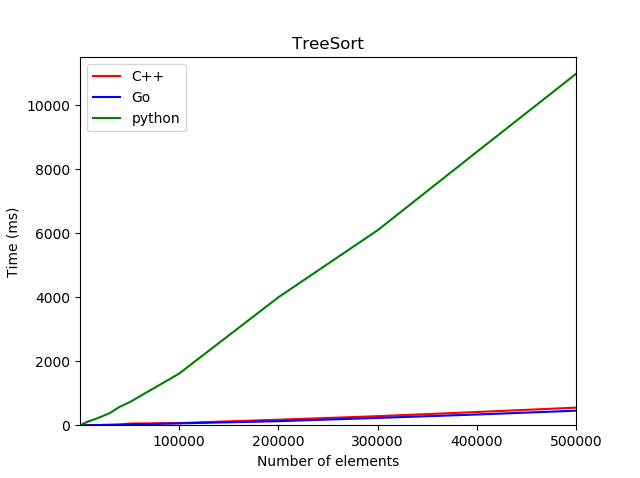
\includegraphics[width=12cm]{img/treeSort_1.png}
            \caption{Estrategia que sigue algoritmo para ordenar una secuencia S de n elementos}
            \label{fig:treesort}
        \end {figure}
    \begin{table}[]
        \begin{tabular}{|c|c|c|c|c|c|c|c| }
            \hline
            \multicolumn{8}{|c|}{Algoritmo: Tree Sort} \\ \hline
            \multicolumn{4}{|c|}{} & \multicolumn{4}{c|}{Lenguaje: C++} \\ \hline
              N de Datos &     t1    &  t2         &  t3          &   t4        &    t5     &   Promedio(t)       & desv. s. \\ \hline
            100   & 0.0345  &   0.0215  &   0.0282   &  0.0198   & 0.0248  & 0.02576  & 0.005850897 \\ \hline
            1000   & 0.2949  &	0.2878  &	0.2575   &	0.2509   & 0.3067  & 0.27956  & 0.024227216 \\ \hline
            2000   & 0.5418  &	0.6543  &	0.4691   &	0.8348   & 0.4672  & 0.59344  & 0.154937287 \\ \hline
            3000   & 1.2841  &	1.3463  &	0.7256   &	0.761    & 1.2948  & 1.08236  & 0.310662217 \\ \hline
            4000   & 1.4992  &	0.9804  &	1.2329   &	2.0372   & 1.1113  & 1.3722   & 0.418131122 \\ \hline
            5000   & 3.241   &   1.7043  &	1.6303   &	2.3498   & 1.629   & 2.11088  & 0.70048675  \\ \hline
            6000   & 2.3611  &	3.3129  &	4.3816	 &  2.7473   & 3.162   & 3.19298  & 0.761382471 \\ \hline
            7000   & 2.6891  &	3.2629  &	2.348	 &  2.3321   & 3.9669  & 2.9198   & 0.69636647  \\ \hline
            8000   & 7.2664  &	3.7294  &	8.6777   &	4.3366   & 5.2377  & 5.84956  & 2.071491642 \\ \hline
            9000   & 3.2077  &	3.1763  &	4.7729   &	3.4111   & 3.5677  & 3.62714  & 0.659954353 \\ \hline
            10000   & 3.5995  &	3.7944  &	3.8475   &	3.9555   & 7.1328  & 4.46594  & 1.496399306 \\ \hline
            20000   & 8.9341  &	12.2247 &	22.0834  &  9.514    & 9.0016  & 12.35156 & 5.605305854 \\ \hline
            30000   & 20.4284 &	15.7075 &   14.5408  &  16.3092  & 15.609  & 16.51898 & 2.276363981 \\ \hline
            40000   & 24.0826	&   23.9909 &	33.5676  &  22.5173  & 26.759  & 26.18348 & 4.402227591 \\ \hline
            50000   & 122.234	&   42.6545 &	44.3492  &  37.6127  & 39.9763 & 57.36534 & 36.35353237 \\ \hline
            100000  & 70.2404	&   77.7421 &	78.2011  &  70.5764  & 77.8051 & 74.91302 & 4.117612814 \\ \hline
            200000   & 174.7876&	193.7067&	172.2818 &	172.4993 & 180.8891& 178.8329 & 9.011849659 \\ \hline
            300000   & 286.8869&	287.1223&	310.3984 &	279.5616 & 280.2003& 288.8339 & 12.57241663 \\ \hline
            400000   & 404.6286&	437.1003&	426.6823 &	414.3129 & 413.0981& 419.16444& 12.74599799 \\ \hline
            500000   & 545.8179&	552.81  &	560.67   &	551.5422 & 565.9059& 555.3492 & 7.930026684 \\ \hline
            \end{tabular}
            \caption{Tabla de resultados Tree Sort con C++}
        \label{tab:treeSortC}
    \end{table}
	\begin{table}[]
        \begin{tabular}{|c|c|c|c|c|c|c|c| }
            \hline
            \multicolumn{8}{|c|}{Algoritmo: Tree Sort} \\ \hline
            \multicolumn{4}{|c|}{} & \multicolumn{4}{c|}{Lenguaje: GO} \\ \hline
              N de Datos &     t1    &  t2         &  t3          &   t4        &    t5     &   Promedio(t)       & desv. s. \\ \hline
100	    &0	    &0	    &0	        &0	    &0	    &0	      &0              \\ \hline
1000	&0	    &0	    &0	        & 0.5229&0	    &0.10458  &0.233847989     \\ \hline
2000	&1.0602	&0	    & 0.5173	&0.5213	&0.6305	&0.54586  &0.377853004\\ \hline
3000	&0.5163	&0.5263	& 0.5168	&1.0277	&0.4843	&0.61428  &0.231653733\\ \hline
4000	&1.4224	&2.1089	& 1.9989	&1.9995	&1.5577	&1.81748  &0.305999987\\ \hline
5000	&1.5459	&1.4908	& 0.9963	&1.7008	&1.8522	&1.5172	  &0.323570479\\ \hline
6000	&2.5209	&2.6206	& 2.9977	&2.2495	&1.5574	&2.38922  &0.536789164\\ \hline
7000	&3.6788	&9.0697	& 4	2.9965	&1.6009	&4.26918&4.26918    &2.837491464\\ \hline
8000	&2.0718	&2.0822	& 4.7402	&5.9971	&6.4824	&4.27474	&2.104585229\\ \hline
9000	&2.0692	&2.8883	& 6.0346	&4.5788	&4.0877	&3.93172	&1.534833267\\ \hline
10000	&8.5031	&7.0278	& 7.0258	&8.9303	&3.0253	&6.90246	&2.33117331\\ \hline
20000	&16.9883&	9.9934	& 11.4141	&11.2215	&10.4236	&12.00818	&2.843572749\\ \hline
30000	&20.9716&	21.9881	& 16.9907	&19.2206	&15.989	    &19.032	    &2.547690131\\ \hline
40000	&17.9895&	21.9853	& 20.9874	&21.9866	&22.9862	&21.187	    &1.922082861\\ \hline
50000	&33.9807&	29.9834	& 28.9829	&31.979	    &26.983	    &30.3818	&2.700491356\\ \hline
100000	&60.0404&	61.9663	& 63.9625	&53.97	    &72.955	    &62.57884	&6.901271991\\ \hline
200000	&116.2649&	130.0599&	145.3944 &140.5367	&129.0323	&132.25764	&11.31501115\\ \hline
300000	&214.4081&	218.5863&	282.0565 &201.3208	&253.0039	&233.87512	&33.01458859\\ \hline
400000	&305.4279&	307.92	& 367.4944	 &341.7326	&384.1765	&341.35028	&35.09183418\\ \hline
500000	&419.8142&	429.1118&	493.0747 &515.5093	&442.0059	&459.90318  & 42.03551579\\ \hline


       \end{tabular}
       \caption{Tabla de resultados Tree Sort con GO}
        \label{tab:treeSortC}
   \end{table}
	%\clearpage
	%\bibliographystyle{apalike}
	%\bibliographystyle{IEEEtranN}
	%\bibliography{bibliography}
		

	\begin{table}[]
        \begin{tabular}{|c|c|c|c|c|c|c|c| }
            \hline
            \multicolumn{8}{|c|}{Algoritmo: Tree Sort} \\ \hline
            \multicolumn{4}{|c|}{} & \multicolumn{4}{c|}{Lenguaje: Python} \\ \hline
              N de Datos &     t1    &  t2         &  t3          &   t4        &    t5     &   Promedio(t)       & desv. s. \\ \hline
100	    &0.015624285	&0	        &0.001001835	&0.000999928	&0	        &3.525209427	&6.782077381 \\ \hline
1000	&0.008558035	&0.003997564	&0.004995108	&0.004993439	&0.010315895	&6.572008133	&2.718788759\\ \hline
2000	&0.019988537	&0.026985168	&0.028544664	&0.011993408	&0.021991014	&21.90055847	&6.553873617\\ \hline
3000	&0.024986029	&0.042976379	&0.049971104	&0.049968719	&0.079953671	&49.57118034	&19.82003258\\ \hline
4000	&0.040974855	&0.091937304	&0.045972109	&0.070964336	&0.067958117	&63.56134415	&20.60862468\\ \hline
5000	&0.044970989	&0.11288166	&0.042973995	&0.101940393	&0.09394598	&79.34260368	&32.98814407\\ \hline
6000	&0.070955515	&0.071353912	&0.058964968	&0.099941492	&0.108936548	&82.03048706	&21.29203294\\ \hline
7000	&0.091950655	&0.099225044	&0.135372639	&0.132360697	&0.10193944	&112.1696949	&20.16856982\\ \hline
8000	&0.120291233	&0.094572067	&0.080644131	&0.139489412	&0.112987995	&109.5969677	&22.82235213\\ \hline
9000	&0.113935947	&0.173901558	&0.073012352	&0.108042202	&0.212877989	&136.3540096	&56.08482712\\ \hline
10000	&0.132925034	&0.090055466	&0.129489422	&0.1939466	&0.133127928	&135.9088898	&37.17781267\\ \hline
20000	&0.315265894	&0.239135265	&0.208152771	&0.246989012	&0.255201578	&252.948904	&39.12004677\\ \hline
30000	&0.378284216	&0.381990671	&0.358812094	&0.447550774	&0.349073887	&383.1423283	&38.49024037\\ \hline
40000	&0.55368185	&0.62367034	&0.560783863	&0.627627611	&0.533614874	&579.8757076	&42.97934242\\ \hline
50000	&0.716868401	&0.73401022	&0.728899479	&0.708563566	&0.729392529	&723.5468388	&10.50482242\\ \hline
100000	&1.756626368	&1.585929394	&1.614357233	&1.669086695	&1.468574524	&1618.914843	&106.292876\\ \hline
200000	&3.741744757	&3.7024014	&3.825145483	&3.708697319	&5.033451557	&4002.288103	&578.508426\\ \hline
300000	&6.054645538	&5.865937948	&6.147264957	&5.924173594	&6.492034435	&6096.811295	&246.7950222\\ \hline
400000	&8.224924326	&8.243051291	&8.770008802	&8.109434605	&9.380488396	&8545.581484	&531.9790418\\ \hline
500000	&9.972488165	&11.47141552	&10.28874731	&10.39334488	&12.78968287	&10983.13575	&1156.877989\\ \hline

       \end{tabular}
   \end{table}


   \section{Resultados}
   \begin{itemize}
     \item  En las pruebas realizadas para el Algoritmo Quick Sort, se obtuvo tiempos de ejecución menores para el código desarrollado en lenguaje de programación Golang, y tiempos de mayor valor en la ejecución del código en lenguaje de programación Python.
     \item	Se observó que, para tamaños de entrada menores a 10 000 datos, los tiempos de ejecución son inconsistentes, al ejecutar el código del algoritmo Quick Sort en lenguaje Golang, presentándose en reiteradas oportunidades valores de cero.
     \item	En la ejecución del algoritmo Quick Sort, los valores de desviación estándar son mayores al ejecutar el código en lenguaje Python, y presentan valores menores al usar el código en C++. Para las pruebas realizadas en Python se observa que los valores de desviación estándar van en aumento respecto al tamaño de la entrada, en el caso del lenguaje Golang y C++, estos valores se incrementan desde 100 000 y 20 000 datos, respectivamente.
     \item  Los programas en lenguaje compilado (C++) presenta un mejor desempeño en cuanto se presenta mayor cantidad de datos que un programa en lenguaje interpretado (Python)
   \end{itemize}

   \section{Referencias}

\end{document} 